\chapter{Quench Localization Problem (\qlp)}
\label{chp:qlp}
This chapter is dedicated to the resolution of the Quench Localization Problem, as we did for \qrp,
we will discuss:
\begin{inparaenum}[(i)]
	\item some of the preprocessing we have done, specific for the labels,
	\item the first approaches with clustering, and finally,
	\item the results obtained, just like we did in \Cref{sec:results-qrp}
\end{inparaenum}.
\section{Problem description}
\section{Data preprocessing}
\label{sec:qlp-preprocessing}
Since the essential difference between the dataset used for \qlp\ and the dataset used for \qrp\,
are the labels, in this section we will concentrate on the considerations arisen from the analysis
of the new labels and the distribution of the points in a bidimensional space. Once more, we will be
splitting the section in different subsections, one for each attribute in the dataset.

\subsubsection{\an}
The correlation with the labels has been plotted in \Cref{fig:an-lcorr-qlp}, as we can see, \an is
correlated very strongly with coils $0$ and $2$, while the correlation is basically non-existent in the
case of coils $1$ and $3$. If we remind ourselves of the correlation existing among the harmonics,
shown in \Cref{fig:an-corr}, we can see that:
\begin{itemize}
	\item Contrarily to what we discovered in \Cref{sec:qrp-preprocessing}, the correlation
	      between harmonic number $2$ and the solution is not strong anymore (for none of the
	      coils);
	\item Now we have a strong correlation for harmonics number $1$ and $3$ (which are very
	      strongly correlated with each other, see \Cref{fig:an-corr}, therefore we will not be able
	      to use them together);
\end{itemize}
A potential dataset could be constructed using a primary odd harmonic (like $1$ or $3$), the
harmonic performing the best among $4, 8$ and $12$ (which are all strongly correlated, see
\Cref{fig:an-corr}) and finally another harmonic between the ones that have been left out. Due to
the very low correlation between the \an\ and the labels for coil $1$ and $3$ we didn't really
consider it as an attribute worth exploring.

\begin{figure}[!h]
	% Font size = 70
	\centering
	\begin{subfigure}{0.49\linewidth}
		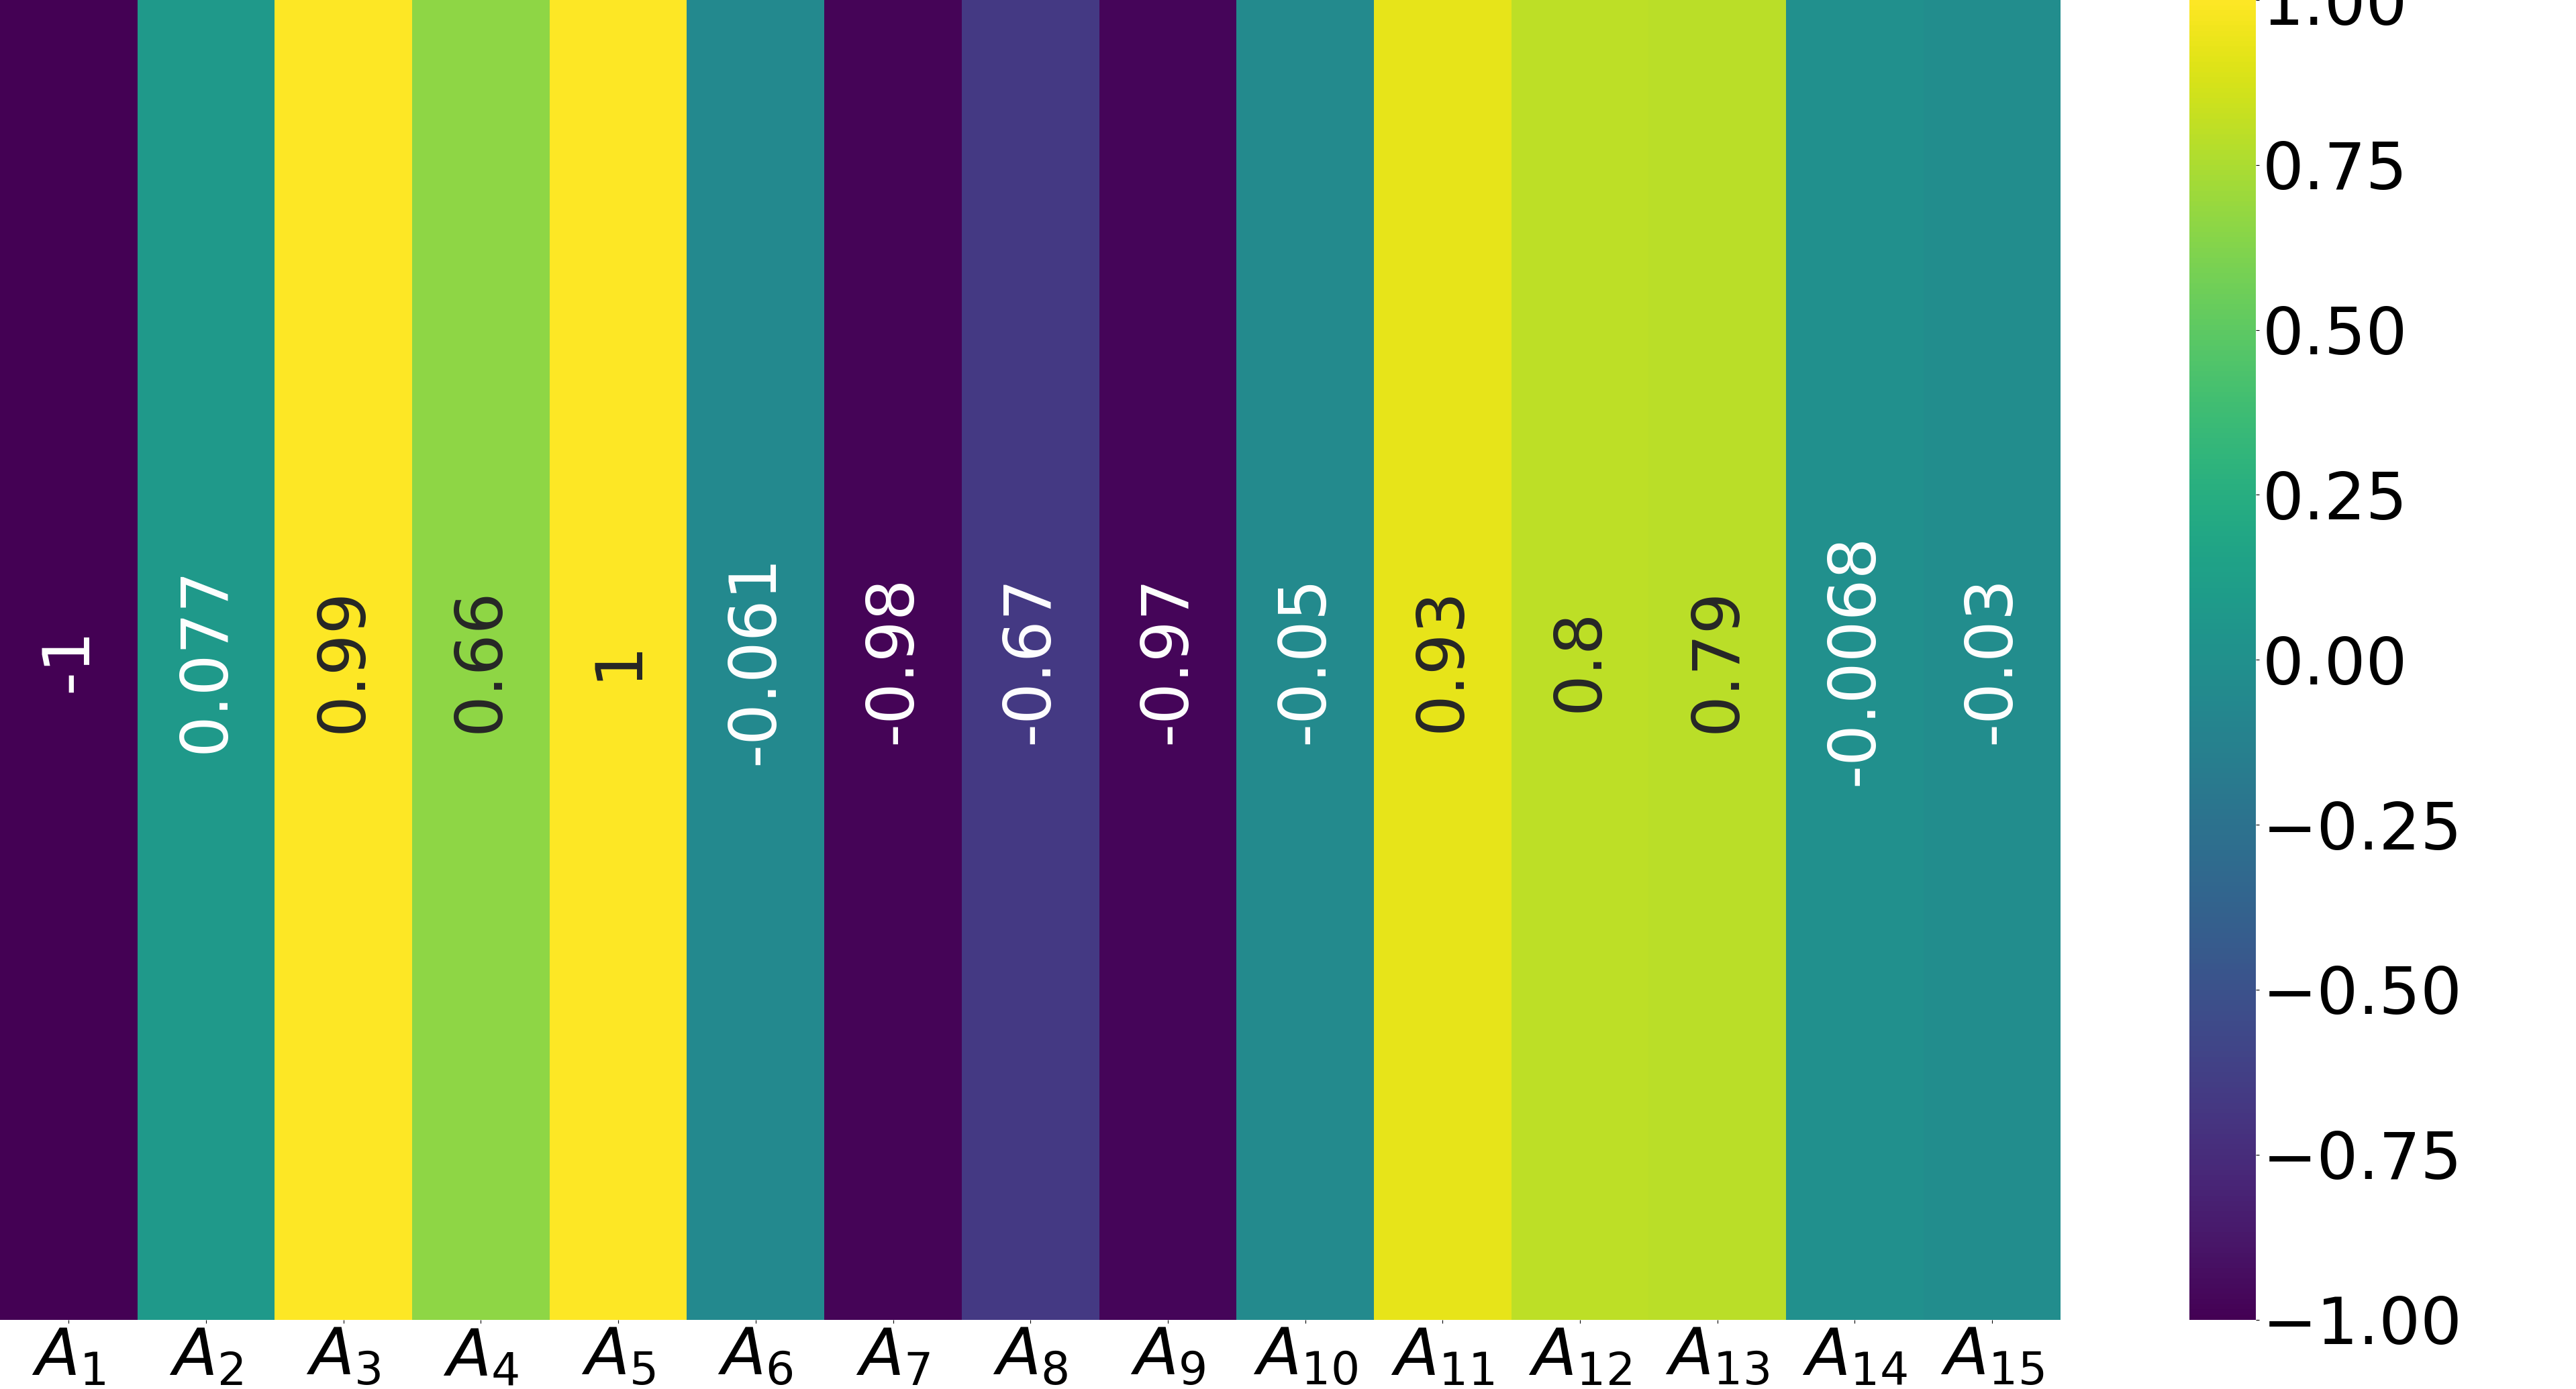
\includegraphics[width=\linewidth]{img/qlp_corr/An_coil0.png}
		\subcaption{Correlation with coil $0$}
	\end{subfigure}
	\begin{subfigure}{0.49\linewidth}
		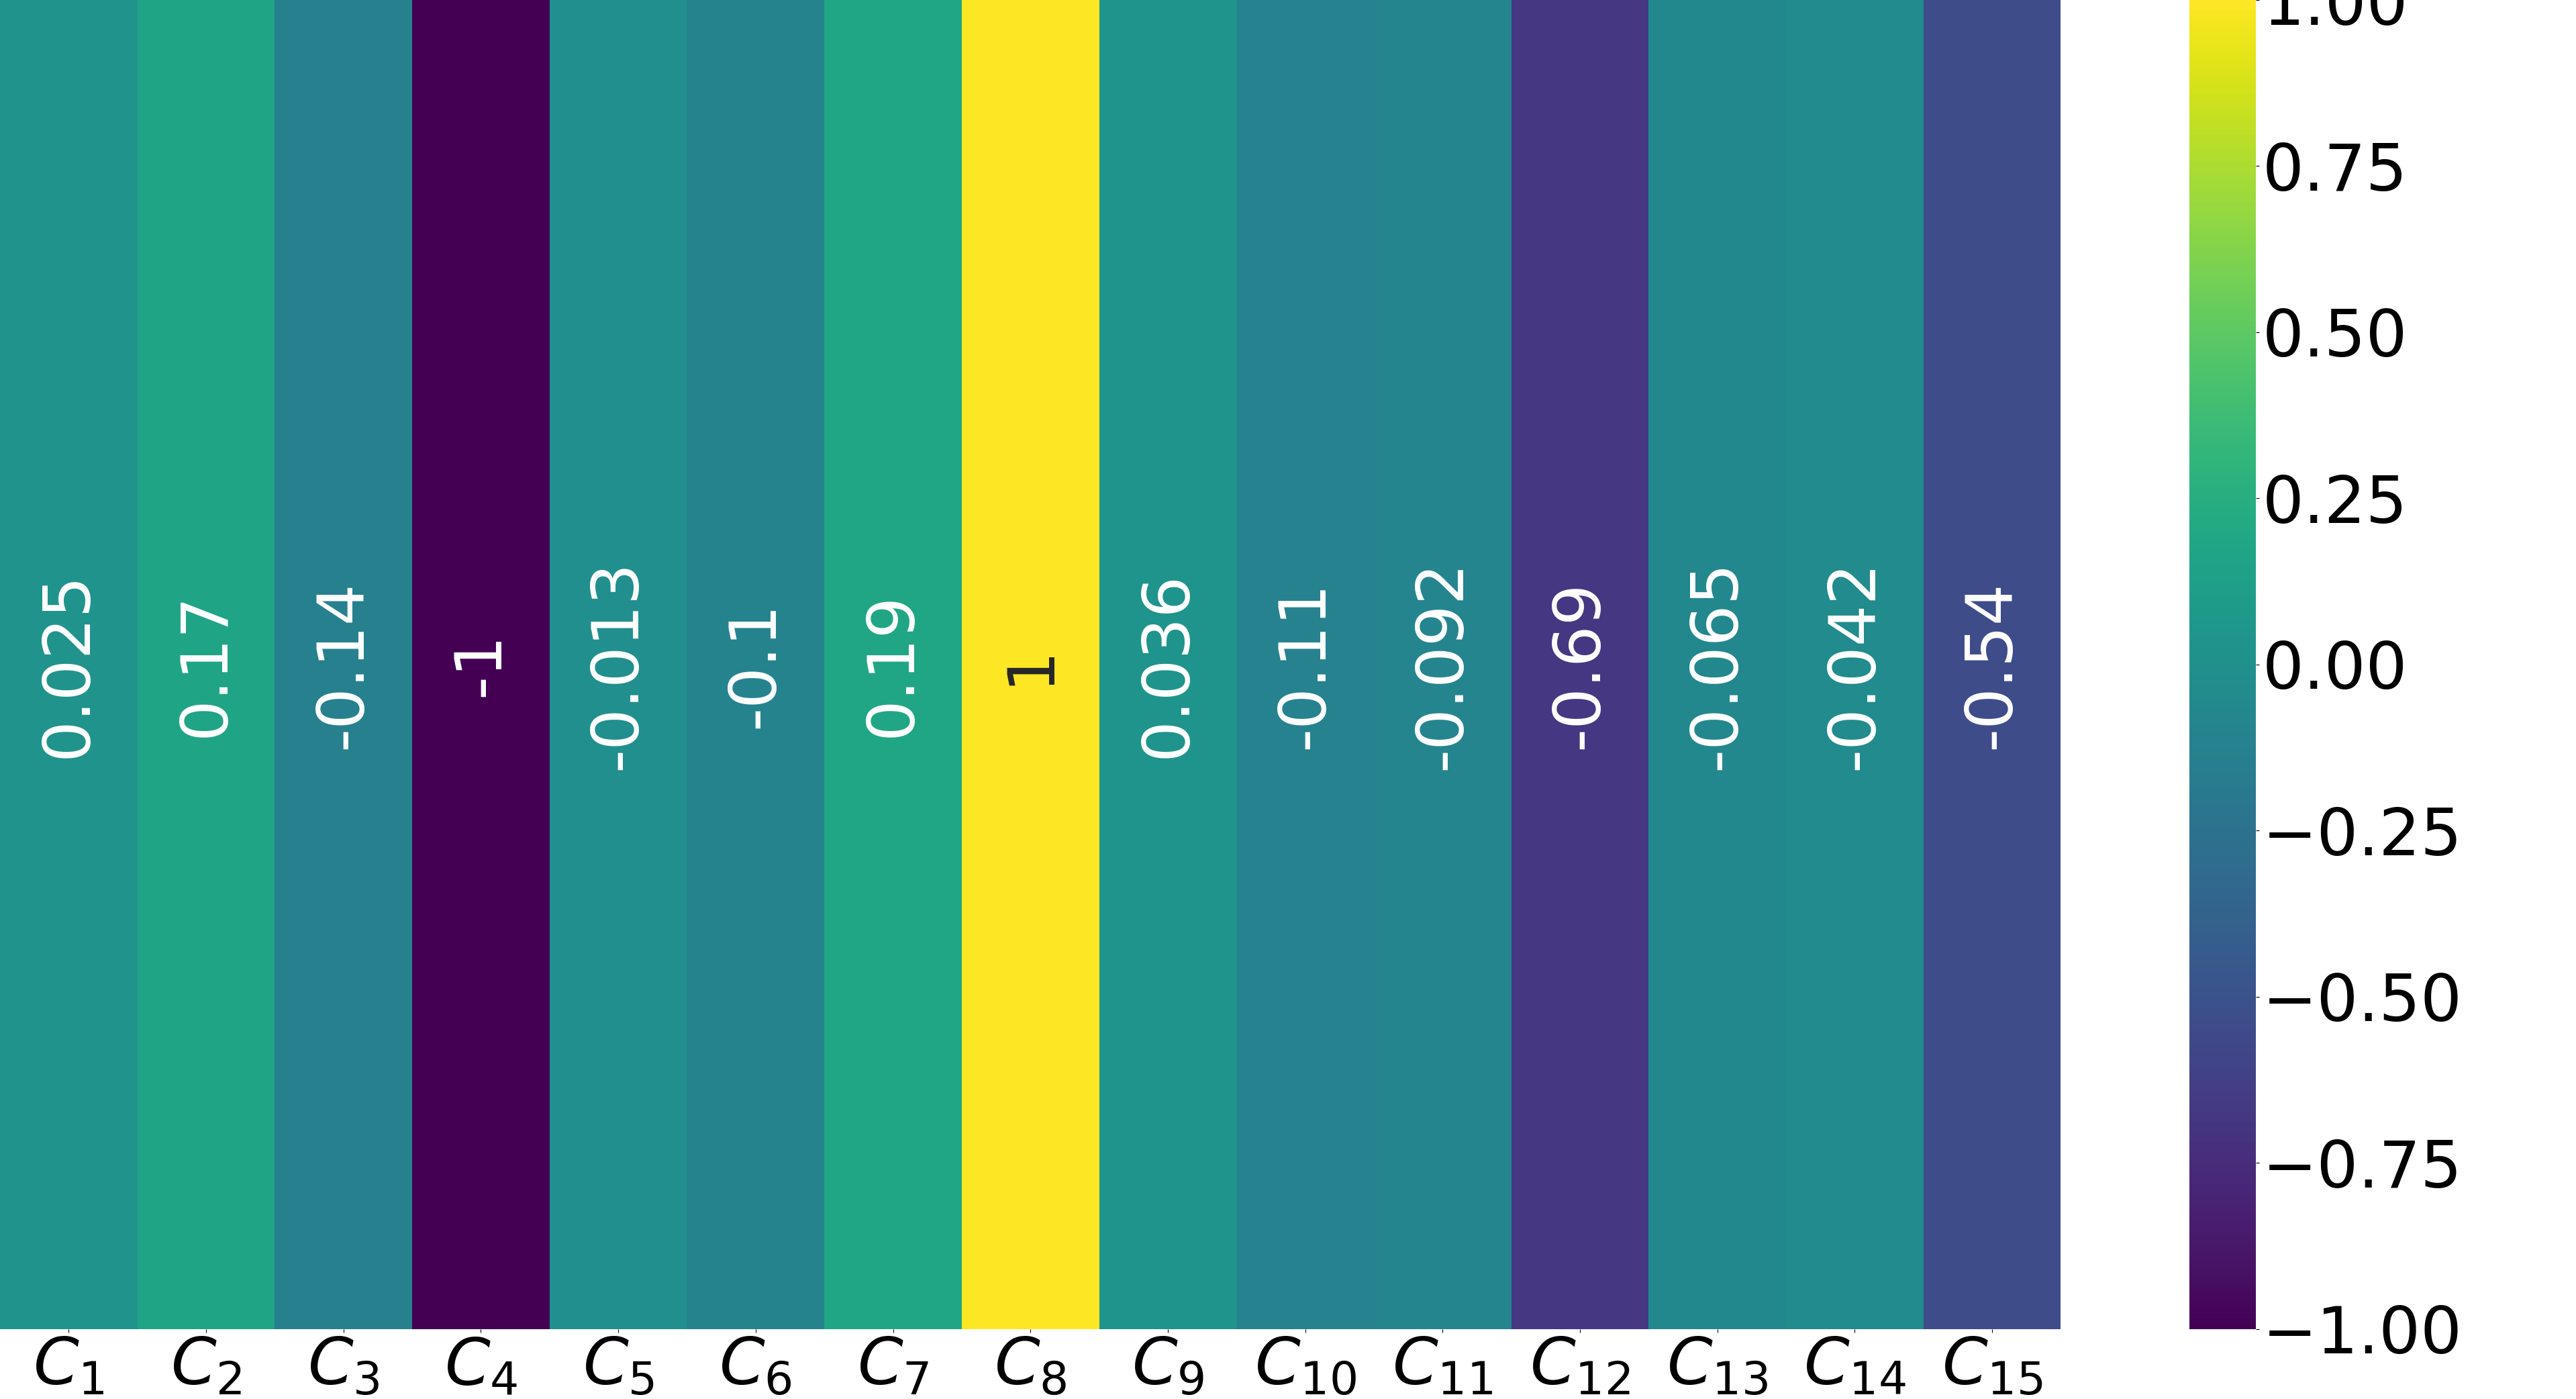
\includegraphics[width=\linewidth]{img/qlp_corr/An_coil1.png}
		\subcaption{Correlation with coil $1$}
	\end{subfigure}
	\begin{subfigure}{0.49\linewidth}
		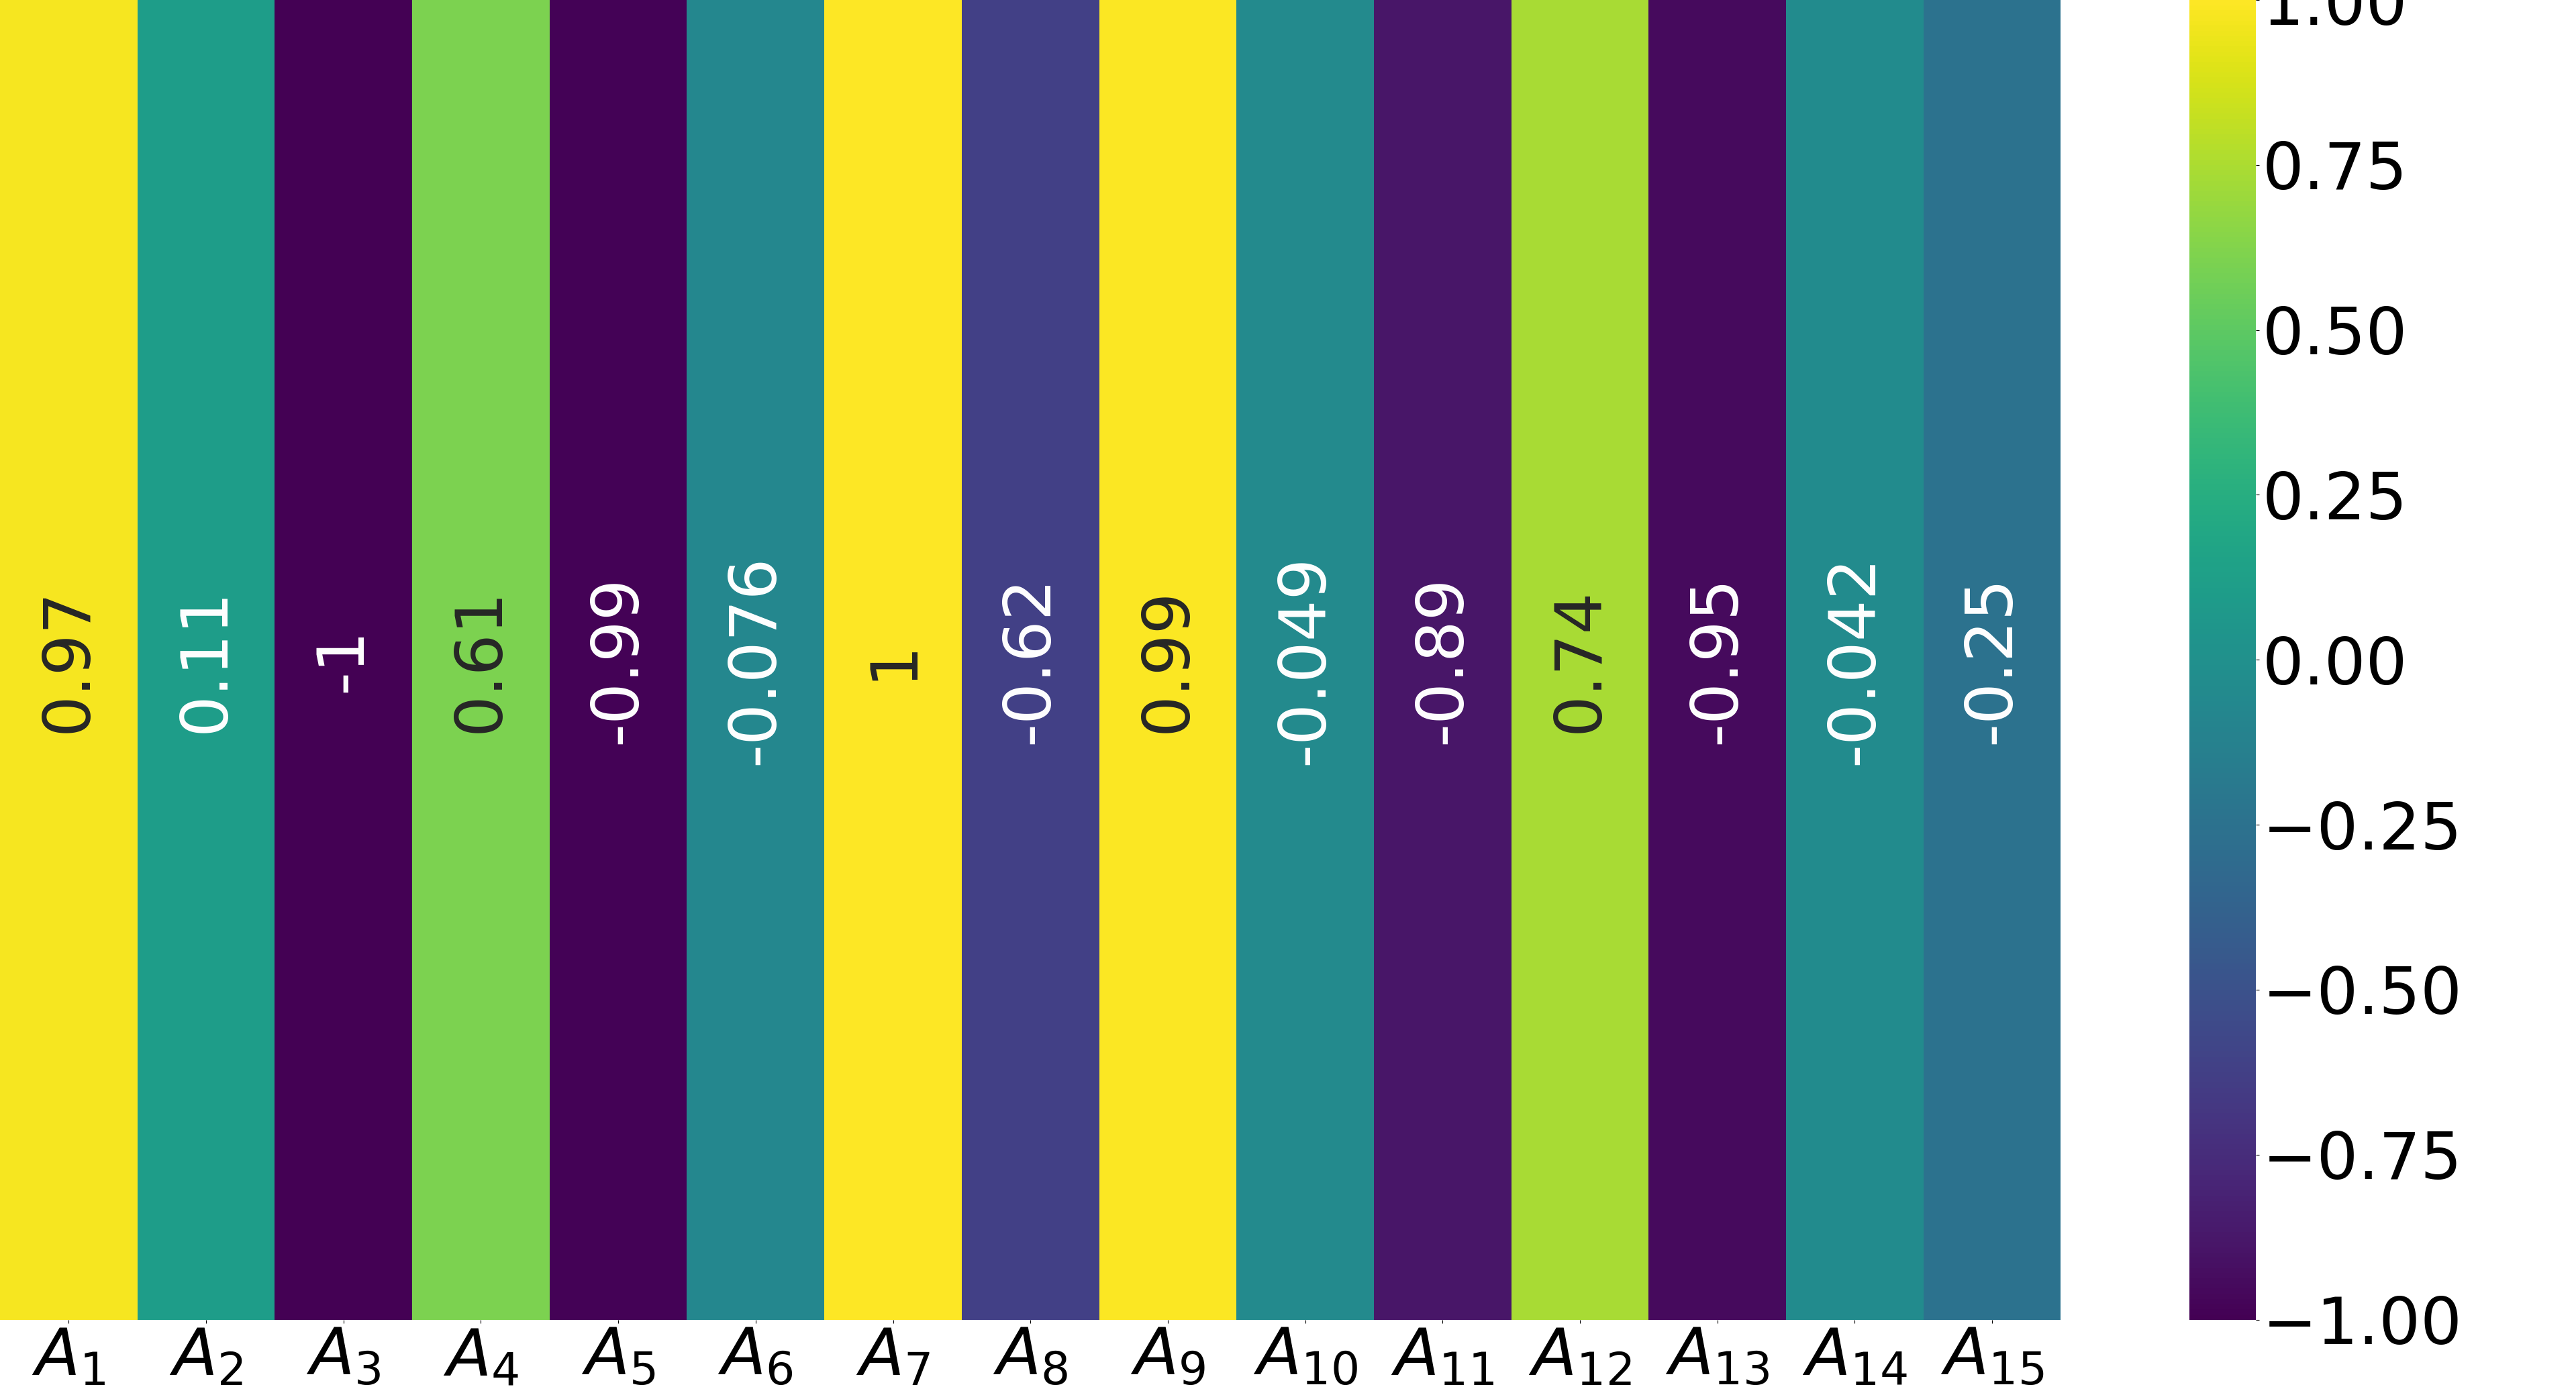
\includegraphics[width=\linewidth]{img/qlp_corr/An_coil2.png}
		\subcaption{Correlation with coil $2$}
	\end{subfigure}
	\begin{subfigure}{0.49\linewidth}
		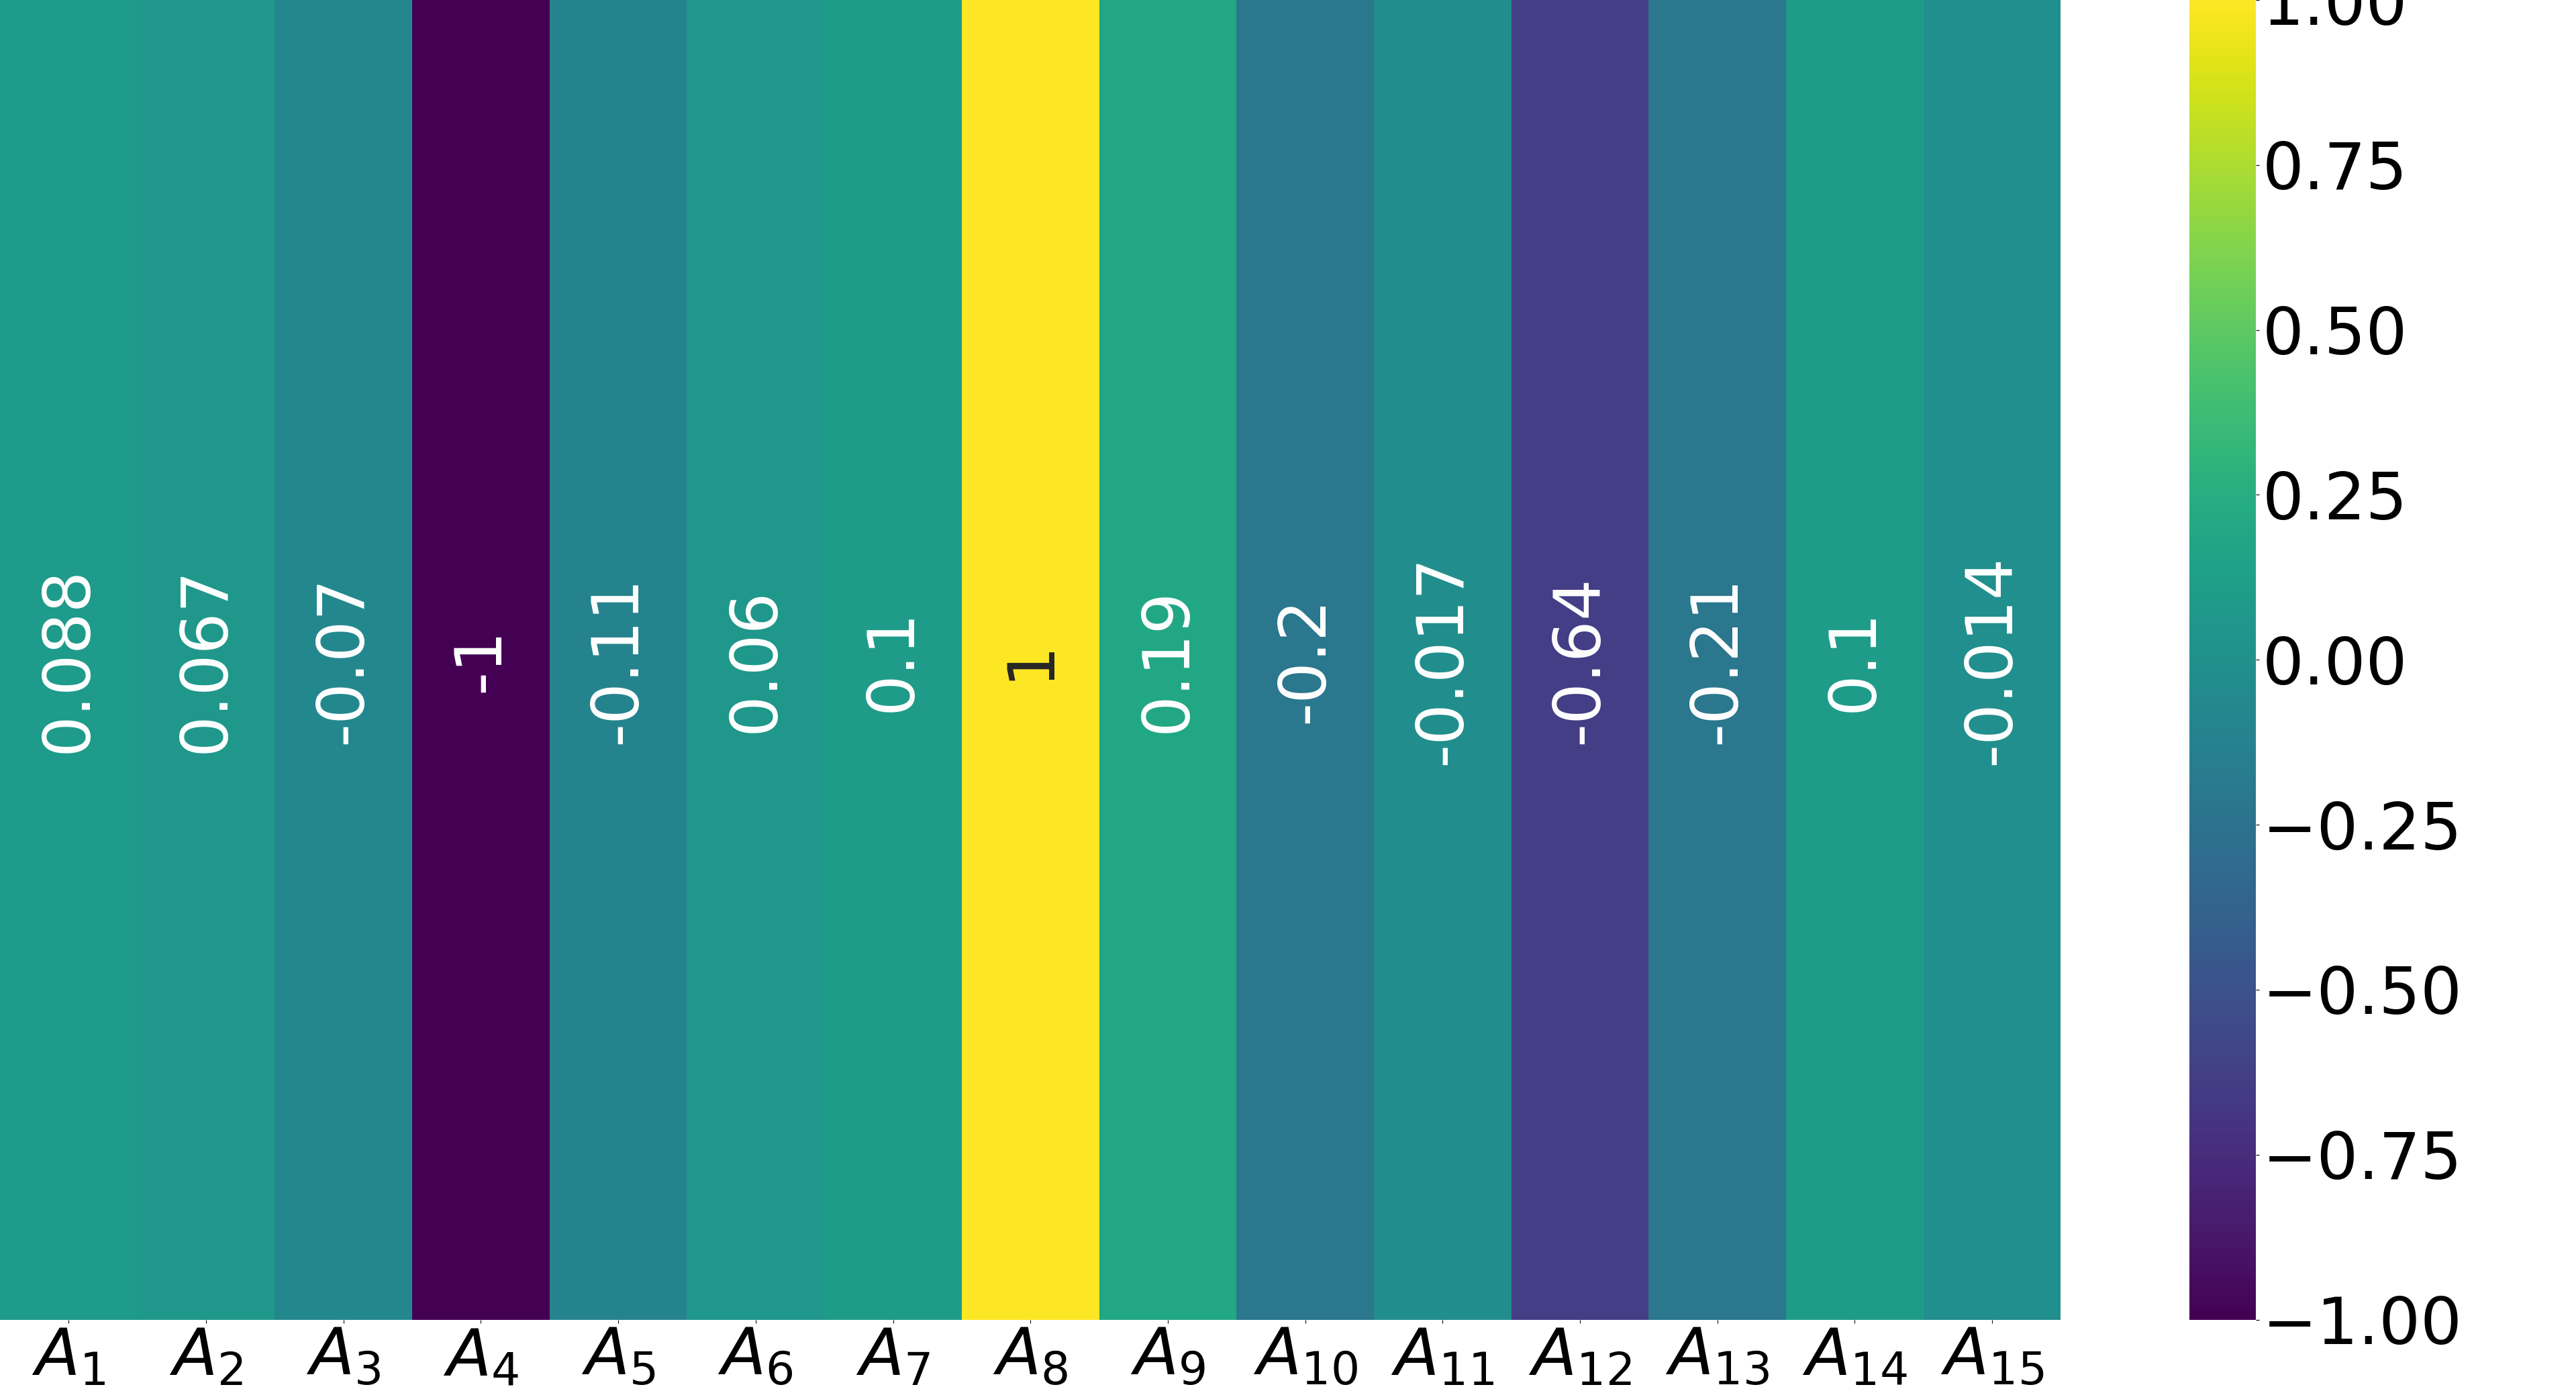
\includegraphics[width=\linewidth]{img/qlp_corr/An_coil3.png}
		\subcaption{Correlation with coil $3$}
	\end{subfigure}
	\caption{Correlation between the harmonics of the \an\ attribute and the labels for \qlp.}
	\label{fig:an-lcorr-qlp}
\end{figure}

\subsubsection{\bn}

\subsubsection{\cnmod}

\subsubsection{\phin}

\section{First approaches using Clustering}
\section{Extension of the QRP models}
\section{Results}
